\section{Problem Overview}

The objective of this project is to address a multi-class news article classification task, where each document must be assigned to one of seven topical categories. The data consists of real-world online news articles provided in raw HTML format, characterized by heterogeneous sources, noisy markup, incomplete metadata, and strong editorial regularities. Performance is evaluated using macro-averaged F1 score, in order to ensure balanced behavior across all classes.

A preliminary exploratory analysis is conducted to identify which signals are informative, redundant, or structurally biased, with the purpose of motivating subsequent preprocessing and modeling choices.

\paragraph{Temporal Metadata and Redundancy}
The \textit{timestamp} attribute contains missing values (approximately \textbf{34.7\%}, corresponding to 27{,}750 out of 80{,}000 records) and exhibits a coarse temporal granularity, with articles concentrated in a limited set of publication years. No deterministic relationship is observed between finer temporal resolutions (month or day) and the target labels.

An auxiliary experiment shows that the publication year can be predicted directly from the raw article text—including HTML structure—with an accuracy of approximately \textbf{64.0\%}. This performance is well above chance level, indicating that temporal information is implicitly encoded in linguistic and editorial patterns. As a consequence, the explicit timestamp is considered a largely redundant signal and is excluded from the feature set.


\begin{figure}[t]
	\centering
	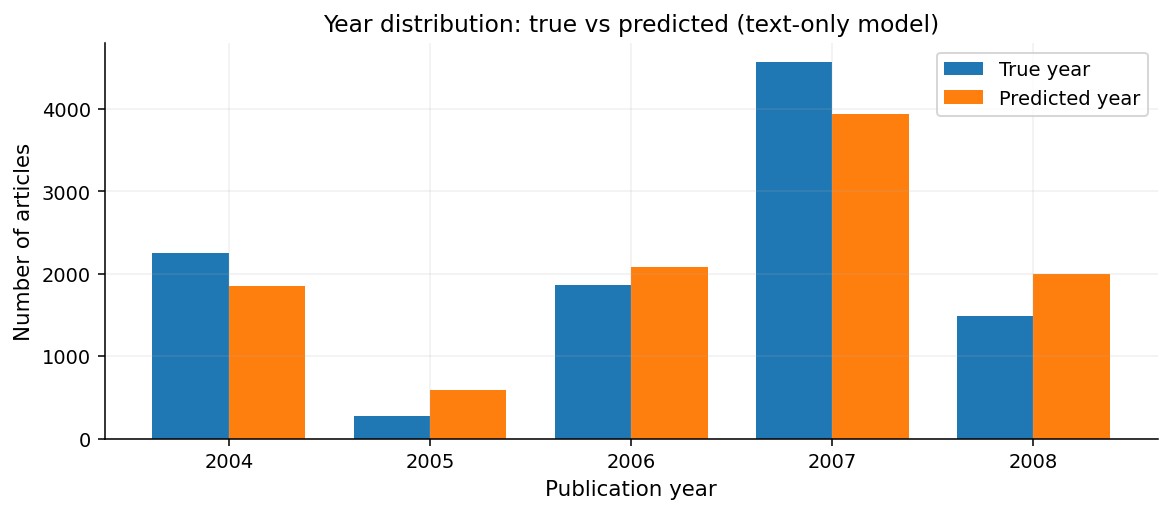
\includegraphics[width=\linewidth]{FIGURES/figure1_year_prediciton.png}
	\caption{Distribution of publication years in the development set and corresponding predictions obtained from a text-only classifier. The strong alignment between true and predicted distributions indicates that temporal information is implicitly encoded in lexical and editorial patterns.}
	\label{fig:year_prediction}
\end{figure}
\paragraph{Non-informative Metadata}
The \textit{page\_rank} feature displays an approximately uniform distribution and does not exhibit a meaningful correlation with the target labels. Empirical checks confirm that its inclusion does not lead to measurable performance improvements, and the feature is therefore discarded.

\paragraph{Structural Ambiguity}
The dataset contains duplicated or republished articles
with identical title--article pairs assigned to different labels
(\textbf{6.87\%} of the development set). This introduces intrinsic ambiguity that defines an upper bound on achievable performance and motivates the use of macro-averaged F1 score as the primary evaluation metric.

\paragraph{Editorial Bias and Source Informativeness}
A strong dependency is observed between article source and target labels, reflecting editorial specialization across publishers. Encoding the source information via one-hot representations yields a strong linear baseline and highlights the presence of near-deterministic editorial cues. This observation motivates the exploration of modeling strategies that explicitly distinguish between structurally deterministic and semantically ambiguous documents.

\textbf{[FIGURE 2 HERE: Source $\times$ Label heatmap]}

\paragraph{Implications}
Overall, the dataset combines noisy HTML-heavy text, incomplete or redundant metadata, and strong editorial regularities. These properties suggest a progressive modeling approach that exploits high-confidence structural signals early, while reserving more expressive models for genuinely ambiguous samples.
